\documentclass[../main]{subfiles}
\begin{document}

\graphicspath{{../figures/}}

\section{提案手法}


\subsection{提案手法のコンセプト}
本研究では,移動ロボットにマイクを搭載し,ロボットの自己位置座標ごとに聞こえる正常音を予測し,観測音との差分から異常音源の座標を推定する手法を提案する.
これは,現場の点検員が異常音を聞き分ける際に,各地点での正常音の記憶と比較して異常音を判別することから着想を得た.
また,正常音との比較を行うことで,各地点での異常な機器由来の音の強さを推定することが可能であり,各位置での強さを用いて異常音源の座標を推定することができる.

\subsection{提案手法の流れ}
まず,検査対象の経路付近の全ての機器が正常に稼働している状態で,ロボットを走行させ,
正常時の座標と音の関係をモデルに学習させる.
運用時には,学習したモデルを用いて学習時と同様の経路を走行させ,閾値処理により経路内の異常音源の有無を判別したのち,異常音源が確認された場合には,その座標を推定する.
運用時のフローチャートを\reffig{flowchart}に示す.
\begin{figure}[tb]
  \centering
  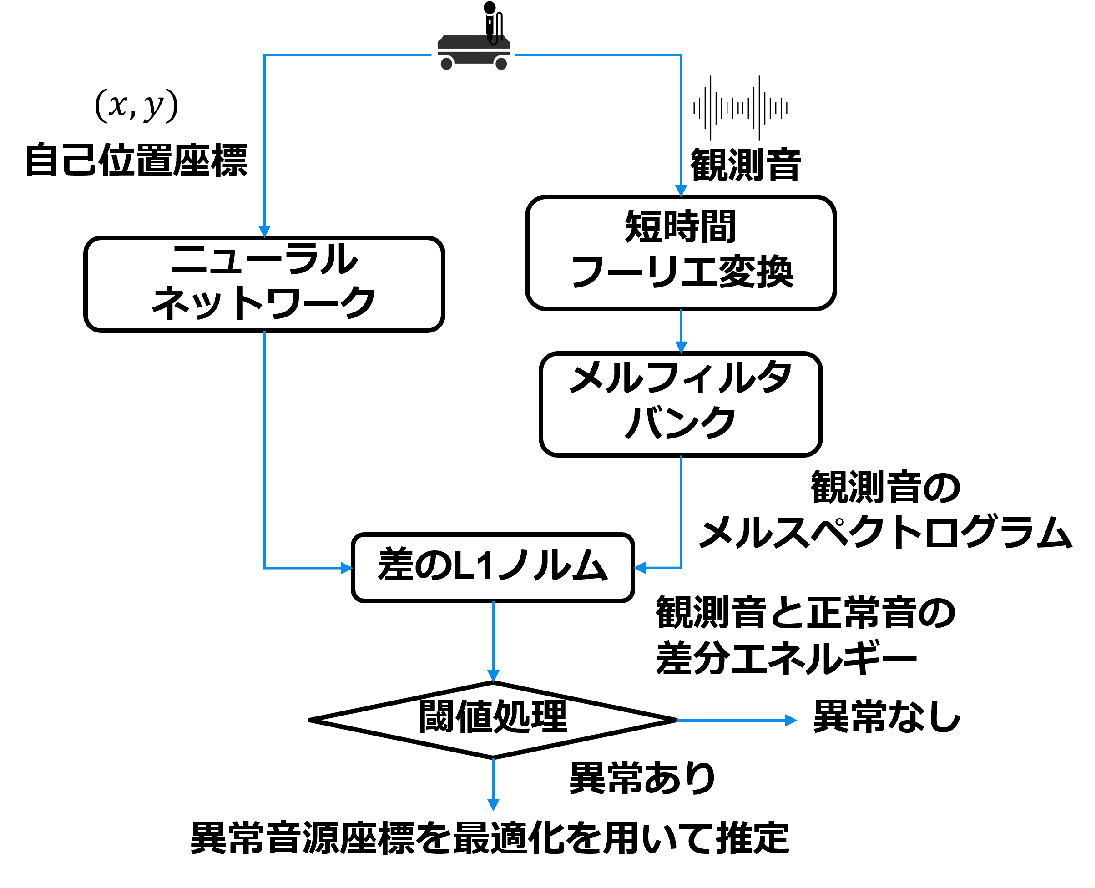
\includegraphics[keepaspectratio, width=1.0\linewidth]{flowchart.pdf}
  \caption{提案手法のフローチャート}
  \labfig{flowchart}
\end{figure}
\subsection{ニューラルネットワークによる正常音のマッピング}
ニューラルネットワーク~\cite{Rumelhart1986}とは,人間の脳の神経細胞を模倣した計算モデルであり,入力層,中間層,出力層から構成され,
各層のノード間の結合には重みが設定されている.
これらの重みを学習することで,入力データから出力データを予測するモデルを構築することができる.
本研究では,ニューラルネットワークを用いて,自己位置の座標を入力とし,その座標に対応する正常音を出力するモデルを構築する.
\subsection{SAMを用いた正常音マッピングモデルの学習}
Sharpness-Aware Minimization(SAM)~\cite{Foret2020}は,
モデル内の重みの更新時に,重みの変化に対する損失関数の変化が小さくなるように重みの更新を行うことで,
汎化性能を向上させることを目的とした最適化手法である.
本研究では,音のマッピングを行うことを提案手法として挙げており,座標の変化に対して出力である音の変化が滑らかになるよう,
モデルの学習を行うために,学習アルゴリズムにSAM Optimizerを用いる.
\subsection{短時間フーリエ変換}
本研究では,座標ごとの正常音をマッピングする手法を提案しているが,音圧のデータは時間ずれの影響を受けやすいことから,音圧の時系列データから
定常的な特徴量を抽出する必要がある.
そのため,音圧の時系列データに対し,短時間フーリエ変換を行い,更にメルフィルタバンクの処理を適用し,次元を削減したメルスペクトログラムを特徴量として用いる.
\subsection{異常音座標の推定手法}
音のエネルギーが距離の二乗に反比例して減衰するという物理的特性にもとづき,異常音源の座標を推定する問題を最適化手法を用いて解く.
異常音源の座標を$\mathbf{x_a}$,音源からの距離が1のとき,マイクで得られる異常音源のエネルギーが$\alpha$とすると,異常音源の座標を推定する問題は以下のように定式化できる.

\begin{equation}
  \underset{\mathbf{x_a}, \alpha}{\arg\min} \sum_i \left| L_1 (\mathbf{m_i^o}, \mathbf{m_i^n}) - \frac{\alpha}{L_2 (\mathbf{x_i}, \mathbf{x_a})^2} \right|,
\end{equation}


$L_1 (\mathbf{m_i^o}, \mathbf{m_i^n})$は正常音と観測音のメルスペクトログラムの差分によって得られる異常音のエネルギーを表し,$L_2 (\mathbf{x_i}, \mathbf{x_a})^2$は異常音源の座標とロボットの自己位置座標間の距離の二乗を表す.

変数として異常音源の座標と比例定数を最適化することで,異常音源の座標を推定することが可能である.

\end{document}
